\documentclass[a4paper,12pt]{report}

% --- Self-contained preamble: no external BOUN style file required, so this
% --- compiles on Overleaf / any TeX Live without styles/fbe_tez.sty. The
% --- bibliography is inlined (thebibliography), so no bibtex run is needed.
\usepackage[utf8]{inputenc}      % Unicode source (Turkish characters)
\usepackage[T1]{fontenc}         % proper Ü, ü, ı, ş, ğ, ç glyphs
\usepackage{lmodern}
\usepackage[a4paper,margin=2.5cm]{geometry}
\usepackage{setspace}
\onehalfspacing
\usepackage{amsmath, amsthm, amssymb}
\usepackage[bottom]{footmisc}
\usepackage{cite}
\usepackage{url}
\usepackage{graphicx}
\usepackage{longtable}
\renewcommand{\labelenumi}{(\roman{enumi})}
\renewcommand{\contentsname}{TABLE OF CONTENTS}
\graphicspath{{figures/}} % Graphics (if any) will be here

% --- Packages used by this report (self-contained: no external image files) ---
\usepackage{booktabs}
\usepackage{array}
\usepackage{xcolor}
\usepackage{tikz}
\usetikzlibrary{shapes.geometric, arrows.meta, positioning, fit, backgrounds, calc}

% Colors for the diagrams
\definecolor{cBg}{HTML}{F4F6F8}
\definecolor{cExtract}{HTML}{DCE9F5}
\definecolor{cExtractB}{HTML}{2C6FAF}
\definecolor{cRenar}{HTML}{E6E0F2}
\definecolor{cRenarB}{HTML}{6A4DA8}
\definecolor{cStore}{HTML}{E7F1E2}
\definecolor{cStoreB}{HTML}{4F8A3A}
\definecolor{cEdge}{HTML}{3A3A3A}

\begin{document}

% Title Page (self-contained, mimics the BOUN report title page layout)
\begin{titlepage}
\centering
\vspace*{0.30\textheight}
{\Large CMPE 492\par}
\vspace{0.7cm}
{\LARGE\bfseries Clear: A Browser Extension for Personalized\\[2pt]
Web Page Renarration with a Vision-Aware\\[2pt]
OpenAI Extraction Pipeline\par}
\vspace{1.6cm}
{\large Berkay Ak\par}
\vspace{1.1cm}
{\large Advisor:\\[4pt] Suzan Üsküdarlı\par}
\vfill
\end{titlepage}

\pagenumbering{roman}
\tableofcontents

\chapter{INTRODUCTION}
\pagenumbering{arabic}

\section{Broad Impact}
The web is the primary medium for information access, yet almost every page is
authored for a single assumed reader. A student skimming for the key claim, a
practitioner who only wants the actionable steps, and a non-native speaker who
needs plainer language all confront the same wall of text. Existing aids---reader
modes, readability extensions, and translation services---apply one fixed
transformation and never ask \emph{who} is reading or \emph{why}.

Clear is a Chrome extension (Manifest V3) that performs personalized web content
\textbf{renarration}: it reshapes a page's text and images to match a configurable
\emph{task} (for example, simpler language, a summary, or an academic register)
and a saved \emph{reading goal} discovered through a short conversation. Rather
than mirroring the source line by line, Clear extracts the page's underlying
facts and rewrites them as a direct explanation of the subject, organized around
what the reader actually wants. The same machinery powers three on-page features:
renarrating a text selection in a floating card, renarrating a whole page into a
clean reading tab, and exporting a self-contained static copy of a page. By
adapting content to the individual reader, the project aims to lower the reading
cost of the web for a broad range of users, including those served by
accessibility guidelines~\cite{wcag}.

\section{Ethical Considerations}
Clear sends page text and, when images are analyzed, page screenshots to the
OpenAI API for processing; users must understand that renarration is a
cloud-assisted operation and that the active page's content leaves the device for
the duration of a request. To limit the footprint, every API request is issued
with \texttt{store: false} so the provider is asked not to retain the
input~\cite{openai}. In contrast, all of the extension's own research and
telemetry data---chat sessions, feedback, preference history, and logs---is kept
\emph{on the device} in a local IndexedDB database with no analytics backend and
no network calls~\cite{indexeddb}, and per-user logging can be disabled entirely.

Like any large-language-model system, the renarration model can reproduce bias or
subtly distort meaning~\cite{parrots}. The system prompt explicitly forbids
fabrication and instructs the model to preserve numbers, named entities, and
contested claims, and to flag irrelevance rather than invent content; a thumbs
up/down and text-correction feedback channel lets users report failures. Finally,
the OpenAI API key is currently inlined into the build and is therefore
extractable from the shipped extension---a known limitation that is documented in
the repository and mitigated operationally by key rotation and usage caps
(Chapter~\ref{ch:impl}).

\chapter{PROJECT DEFINITION AND PLANNING}

\section{Project Definition}
Clear is a single-developer Chrome extension that renarrates web content using
the OpenAI Responses API. It is organized as a two-phase pipeline. The
\emph{extraction} phase reads the visible page (text, sections, and images) and
distills it into a structured list of facts and claims using many small,
parallel model calls bounded by a per-run budget. The \emph{renarration} phase
turns those facts into natural prose shaped by the active task and the saved
reading goal. Around this core, the extension provides a text-selection overlay,
a full-page reading view, a static-site exporter, a reading-goal chatbot, an
options page for configuring tasks and prompts, and a research dashboard backed by
on-device storage. The project also serves as a small research platform for
studying how readers interact with AI-renarrated content.

\section{Project Planning}

\subsection{Project Time and Resource Estimation}
The project is built incrementally by a single developer on consumer hardware,
using an OpenAI API key for inference. Table~\ref{tab:timeline} summarizes the
development phases reflected in the repository history.

\begin{table}[thbp]
\vskip\baselineskip
\caption[Project timeline]{Project development timeline.}
\begin{center}
\begin{tabular}{|c|l|p{8.2cm}|} \hline
\textbf{Phase} & \textbf{Duration} & \textbf{Key Deliverables} \\ \hline
1 & Weeks 1--4 & MV3 extension scaffold, OpenAI Responses API client, text-selection renarration, task data model, options page. \\ \hline
2 & Weeks 5--8 & Two-phase page pipeline: visible-text extraction, full-page renarration into a reading tab, static-site exporter, viewer pages. \\ \hline
3 & Weeks 9--12 & Reading-goal chatbot, budget-bounded map/reduce extraction with vision image curation, on-device research store, feedback, dashboard, security hardening, CI. \\ \hline
\end{tabular}
\label{tab:timeline}
\end{center}
\end{table}

\subsection{Success Criteria}
\begin{enumerate}
\item Functional text-selection renarration in a floating on-page card.
\item Whole-page renarration that covers the page's facts and opens in a clean reading tab.
\item Vision-based image curation that keeps relevant figures and renarrates their captions.
\item A self-contained static-site export with images embedded as data URIs.
\item A reading-goal chatbot that produces a structured goal and applies it to renarration.
\item A configurable task and prompt-template system with create/edit/delete operations.
\item On-device research data collection with feedback capture and JSON/CSV export.
\end{enumerate}

\subsection{Risk Analysis}
Table~\ref{tab:risk} lists the principal risks and the mitigations that are
present in the codebase.

\begin{table}[thbp]
\vskip\baselineskip
\caption[Key risks]{Key risks and mitigations.}
\begin{center}
\begin{tabular}{|p{4.2cm}|c|p{6.4cm}|} \hline
\textbf{Risk} & \textbf{Impact} & \textbf{Mitigation} \\ \hline
Dense pages overflow per-call latency or token limits & High & Per-run budget (wall-clock, tokens, storage); concurrency-limited subagents; one-shot truncation retry with a doubled token budget. \\ \hline
API key extractable from the shipped bundle & High & Documented in \texttt{SECURITY.md}; \texttt{.env} gitignored; key rotation and usage caps; planned per-user key / proxy. \\ \hline
Content-script injection on untrusted pages & Medium & Overlay rendered in a Shadow DOM; \texttt{innerHTML} sinks escaped; final text rendered with \texttt{textContent}. \\ \hline
Renarrated payload exceeds storage quota & Medium & Size-check before writing; explicit storage-write limit with a clear error. \\ \hline
\end{tabular}
\label{tab:risk}
\end{center}
\end{table}

\subsection{Team Work}
This is a solo project; all roles---design, implementation, testing, and
documentation---are handled by Berkay Ak.

\chapter{RELATED WORK}
Mainstream reading aids such as reader modes and readability extensions
(Mercury Reader, Readability) strip layout and boilerplate but apply a uniform
transformation that ignores the reader's intent and background. Web Content
Accessibility Guidelines~\cite{wcag} push toward perceivable, understandable
content, but leave the act of \emph{re-expressing} meaning to authors. The notion
of \emph{renarration}---reformulating content so it reads as if written for a
specific reader---draws on comprehension theory, in which understanding is the
construction of a situation model rather than the decoding of
surface text~\cite{kintsch}. Readability research provides quantitative framing
for ``simpler'' or ``denser'' rewrites~\cite{flesch}.

Large language models make automated renarration practical. Clear uses the
OpenAI Responses API with strict JSON-schema structured outputs to obtain
machine-checkable facts and image verdicts rather than free text~\cite{openai},
and vision inputs let the model read figures and screenshots that pure DOM
parsing misses. Because a single model call cannot reliably and exhaustively
process a long page within latency and token limits, the extraction stage adopts
a \emph{map/reduce} strategy: many small extractions run in parallel and are then
hierarchically merged~\cite{mapreduce}. The whole system is shaped by the
constraints of the Manifest V3 extension platform---a module service worker, a
strict extension-page content security policy, and no persistent background
state~\cite{mv3}. Finally, awareness of model bias and faithfulness risk in
generative rewriting informs the project's guardrails and feedback
channel~\cite{parrots}.

\chapter{METHODOLOGY}

\section{Two-Phase Extract--Renarrate Architecture}
Clear deliberately separates \emph{what the page says} from \emph{how it is
retold}. The extraction phase (\texttt{src/page-flow/extract-page.js}) converts a
live page into a structured knowledge object---a list of typed facts and claims
plus curated sections and images---while the renarration phase
(\texttt{src/page-flow/renarrate-page.js}) consumes only that structured object
to write prose. Separating the phases means the expensive, page-dependent reading
work happens once and can be reused by every output (selection card, full-page
view, static site), and the rewrite step never has to re-parse raw HTML. All
model access goes through a single OpenAI client
(\texttt{src/utils/openai-client.js}) that wraps the Responses API, sends
\texttt{store: false}, and transparently adapts request parameters to the model
family (reasoning models receive a \texttt{reasoning} effort; classic models
receive \texttt{temperature}). The default text and vision model is configurable
via \texttt{.env} and ships as \texttt{gpt-5.5}.

\section{Budget-Bounded Map/Reduce Extraction}
Rather than capping work at a fixed number of segments or images, extraction is
bounded by a single per-run \emph{budget} with three ceilings: wall-clock time
(default 220{,}000\,ms), estimated token spend (default 350{,}000 tokens), and
output storage size (default 8.5\,MB). A planner splits the visible page into
text segments and ranks candidate images; a budget check (\texttt{canDispatch})
gates every subagent call so that coverage degrades gracefully under load instead
of failing. The mapping stage dispatches text subagents and vision subagents
concurrently, each with a small retry that absorbs transient errors and rate
limits. Each text subagent returns strict-schema JSON containing facts, topic,
entities, and key terms. The reduce stage merges results: when the combined facts
already fit the output budget the orchestrator assembles them locally to save a
model call; otherwise a hierarchical, merge-only reducer combines and deduplicates
them. Crucially, coverage is never silently truncated---budget skips and possible
duplicates are recorded as warnings and surfaced to the user.

\section{Vision-Based Image Curation}
Image handling is decoupled from fact extraction. Candidate images are ordered by
a relevance score and sent, strongest first, to vision subagents that return a
keep/drop verdict, a caption, and an optional bonus fact per image. Because the
budget---not a fixed count---decides how many images reach the model, the most
important figures are evaluated even when a page is image-heavy. Kept images are
re-attached to their sections, and their captions are later renarrated to match
the output language and reading goal of the body text.

\section{Prompt and Task System}
Three Markdown prompt templates in \texttt{src/prompts/} are fetched at runtime
through \texttt{chrome.runtime.getURL} and cached: a renarration system prompt
(\texttt{system.md}), a chatbot system prompt (\texttt{chatbot-system.md}), and a
goal-extraction prompt (\texttt{goal-extraction.md}). The renarration system
prompt is assembled from boilerplate plus the active task's instruction and the
saved reading goal, with placeholders \texttt{\{task\}} and
\texttt{\{readingGoal\}} substituted at request time and an explicit
output-language rule appended. Four default tasks ship with the
extension---Simple Language, Detailed Explanation, Academic Style, and
Summary---each defined by a text prompt, an image prompt, and a target length;
all tasks are user-editable. A key design rule, enforced in the prompt, is that
the renarration explains the subject \emph{directly} (``state the information as
facts about the subject'') and avoids meta-attribution such as ``the article
says,'' reserving attribution for genuine quotations and contested claims.

\section{Reading-Goal Discovery via Chatbot}
A multi-turn chatbot (\texttt{src/handlers/chatbot.js}), reachable from the
document overlay, helps the user articulate what they want from a page by asking
one question at a time about goal, depth, focus, and style. On request, a separate
extraction call converts the transcript into a strict JSON reading goal with
fields \texttt{readingGoal}, \texttt{desiredDepth}, \texttt{focusAreas},
\texttt{outputStyle}, \texttt{additionalInstructions}, and a \texttt{language}
code (ISO 639-1). The goal is saved to \texttt{chrome.storage.sync} and becomes
the primary organizing lens for subsequent renarration; the detected language
makes the renarration follow the language the user actually chatted in.

\section{On-Device Research Data Collection}
The extension records anonymized research data---chat sessions, research logs,
feedback events, and preference history---in a local IndexedDB database
(\texttt{src/utils/research-store.js}). This store replaces an earlier
cloud-database client so that data stays on the device with no network calls and
no credentials, and writes are best-effort so a logging failure never breaks a
user-facing feature. Each record carries a stable anonymous user ID and is
indexed by it, enabling per-user export to JSON or CSV from the dashboard.

\chapter{REQUIREMENTS SPECIFICATION}

\section{Use Cases}
Two actors interact with the system: an \emph{End User} who reads and renarrates
pages, and a \emph{Researcher} who reviews collected data.
Table~\ref{tab:usecases} summarizes the use cases and Figure~\ref{fig:usecase}
shows them as a use-case diagram.

\begin{table}[thbp]
\vskip\baselineskip
\caption[Use case summary]{Use case summary.}
\begin{center}
\begin{tabular}{@{}llp{8.6cm}@{}}
\toprule
\textbf{ID} & \textbf{Actor} & \textbf{Description} \\
\midrule
UC-1 & End User & Renarrate a text selection in a floating on-page card. \\
UC-2 & End User & Extract whole-page knowledge (facts, sections, images). \\
UC-3 & End User & Renarrate the full page into a clean reading tab. \\
UC-4 & End User & Export a self-contained static site with embedded images. \\
UC-5 & End User & Discover and apply a reading goal via the chatbot. \\
UC-6 & End User & Create, edit, and delete tasks; edit the prompt template. \\
UC-7 & End User & Give thumbs up/down feedback or a text correction. \\
UC-8 & Researcher & View and export collected research data; toggle logging. \\
\bottomrule
\end{tabular}
\label{tab:usecases}
\end{center}
\end{table}

\begin{figure}[thbp]
\centering
\begin{tikzpicture}[
  every node/.style={font=\footnotesize},
  uc/.style={draw=cExtractB, fill=cExtract, ellipse, minimum width=3.5cm, minimum height=0.95cm, align=center, inner sep=1pt},
  actor/.style={align=center, font=\footnotesize}
]
% Actors
\node[actor] (user) at (0,0) {%
  \begin{tikzpicture}[scale=0.5]
    \draw[thick] (0,0) circle (0.28);
    \draw[thick] (0,-0.28) -- (0,-1.1);
    \draw[thick] (-0.5,-0.6) -- (0.5,-0.6);
    \draw[thick] (0,-1.1) -- (-0.4,-1.7);
    \draw[thick] (0,-1.1) -- (0.4,-1.7);
  \end{tikzpicture}\\ End User};
\node[actor] (res) at (0,-6.6) {%
  
\begin{tikzpicture}[scale=0.5]
    \draw[thick] (0,0) circle (0.28);
    \draw[thick] (0,-0.28) -- (0,-1.1);
    \draw[thick] (-0.5,-0.6) -- (0.5,-0.6);
    \draw[thick] (0,-1.1) -- (-0.4,-1.7);
    \draw[thick] (0,-1.1) -- (0.4,-1.7);
  \end{tikzpicture}\\ Researcher};

% System boundary with use cases
\node[uc] (u1) at (5.2,1.6) {UC-1 Renarrate selection};
\node[uc] (u2) at (5.2,0.5) {UC-2 Extract page};
\node[uc] (u3) at (5.2,-0.6) {UC-3 Renarrate page};
\node[uc] (u4) at (5.2,-1.7) {UC-4 Export static site};
\node[uc] (u5) at (5.2,-2.8) {UC-5 Set reading goal};
\node[uc] (u6) at (5.2,-3.9) {UC-6 Manage tasks/prompt};
\node[uc] (u7) at (5.2,-5.0) {UC-7 Submit feedback};
\node[uc] (u8) at (5.2,-6.6) {UC-8 Export research data};

\begin{scope}[on background layer]
\node[draw=gray, rounded corners, fit=(u1)(u8), inner sep=12pt, label={[gray]above:\textbf{Clear extension}}] {};
\end{scope}

\foreach \u in {u1,u2,u3,u4,u5,u6,u7} \draw[-, gray] (user) -- (\u);
\draw[-, gray] (res) -- (u8);
\end{tikzpicture}
\caption{Use-case diagram. The End User drives the renarration features;
the Researcher reviews and exports on-device data.}
\label{fig:usecase}
\end{figure}

\section{Non-Functional Requirements}
Table~\ref{tab:nfr} lists the key non-functional requirements, each grounded in a
concrete mechanism in the repository.

\begin{table}[thbp]
\vskip\baselineskip
\caption[Non-functional requirements]{Key non-functional requirements.}
\begin{center}
\begin{tabular}{@{}llp{8.0cm}@{}}
\toprule
\textbf{ID} & \textbf{Category} & \textbf{Requirement} \\
\midrule
NFR-1 & Privacy & Research/telemetry data stays on-device in IndexedDB; no analytics backend; logging is user-toggleable. \\
NFR-2 & Security & API requests use \texttt{store: false}; extension-page CSP \texttt{script-src 'self'; object-src 'self'}; overlay isolated in Shadow DOM; output rendered with \texttt{textContent}. \\
NFR-3 & Reliability & Per-run budget (time/tokens/storage); transient-error and truncation retries; run lock; storage size guard; coverage warnings never silently dropped. \\
NFR-4 & Performance/Cost & Optional faster ``bulk'' model; low image-detail default; low reasoning effort for prose; 120\,s request timeout. \\
NFR-5 & Compatibility & Chrome Manifest V3; Node 20 build; Vite bundles only the service worker. \\
NFR-6 & Maintainability & ESLint, Prettier, knip, and Vitest; CI runs build + lint + test on every push and pull request. \\
\bottomrule
\end{tabular}
\label{tab:nfr}
\end{center}
\end{table}

\chapter{DESIGN}

\section{Information Structure}
Two stores hold user-facing state. Synchronized configuration in
\texttt{chrome.storage.sync} contains \texttt{enabled}, \texttt{currentTask}, the
\texttt{tasks} map (each task: \texttt{name}, \texttt{textPrompt},
\texttt{imagePrompt}, \texttt{maxLength}), the editable
\texttt{systemPromptTemplate}, and the structured \texttt{readingGoal}.
Pipeline state in \texttt{chrome.storage.local} holds the anonymous
\texttt{studyUserId}, the most recent \texttt{lastExtraction},
\texttt{lastPageRenarration}, \texttt{lastRenarratedSite}, and
\texttt{lastTextRenarration}, plus chat sessions and the research-logging flag.
Research data lives in an IndexedDB database (\texttt{renarration-research},
version 1) with four object stores---\texttt{chatSessions} (keyed by
\texttt{sessionId}), \texttt{researchLogs} (\texttt{logId}),
\texttt{feedbackEvents} (\texttt{feedbackId}), and \texttt{userPreferences}
(auto-generated \texttt{preferenceId})---each carrying a \texttt{userId} index. The
extraction object is the central artifact: a \texttt{title}, a list of typed
\texttt{facts} (each with a kind, text, optional evidence, confidence, and section
and image references), the curated \texttt{sections} and \texttt{images}, and any
coverage \texttt{warnings}.

\section{Information Flow}
All inter-component communication uses \texttt{chrome.runtime} messages routed by
an \texttt{action} field. A single background service worker is the hub: content
scripts and UI pages send actions, the message handler dispatches them to the
appropriate handler module, and results flow back. Outbound model calls go to the
OpenAI Responses API; persistent state goes to \texttt{chrome.storage} and
IndexedDB. Figure~\ref{fig:flow} shows the main paths.

\begin{figure}[thbp]
\centering
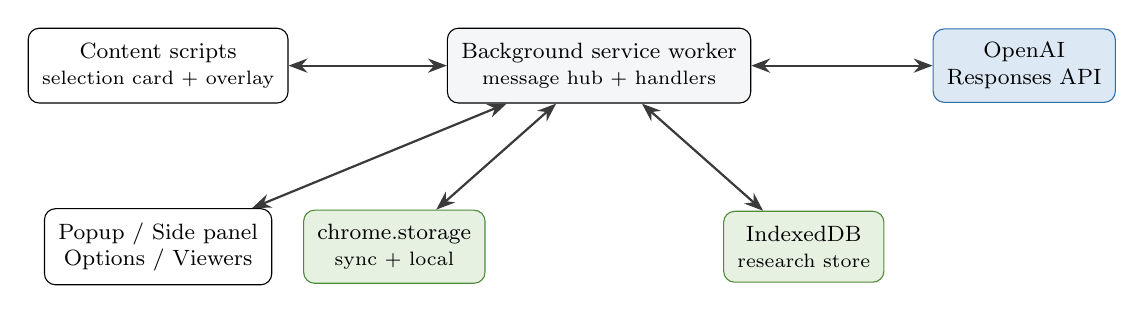
\begin{tikzpicture}[
  every node/.style={font=\footnotesize},
  box/.style={draw, rounded corners, align=center, minimum height=0.95cm, inner sep=5pt, fill=white},
  store/.style={draw=cStoreB, fill=cStore, rounded corners, align=center, minimum height=0.9cm, inner sep=5pt},
  ext/.style={draw=cExtractB, fill=cExtract, rounded corners, align=center, minimum height=0.9cm, inner sep=5pt},
  ar/.style={-{Stealth[length=2.4mm]}, thick, draw=cEdge}
]
\node[box] (cs) at (0,0) {Content scripts\\\scriptsize selection card + overlay};
\node[box, fill=cBg] (sw) at (5.6,0) {Background service worker\\\scriptsize message hub + handlers};
\node[ext] (api) at (11.0,0) {OpenAI\\Responses API};
\node[store] (sync) at (3.0,-2.3) {chrome.storage\\\scriptsize sync + local};
\node[store] (idb) at (8.2,-2.3) {IndexedDB\\\scriptsize research store};
\node[box] (ui) at (0,-2.3) {Popup / Side panel\\Options / Viewers};

\draw[ar, {Stealth[length=2.4mm]}-{Stealth[length=2.4mm]}] (cs) -- (sw);
\draw[ar, {Stealth[length=2.4mm]}-{Stealth[length=2.4mm]}] (sw) -- (api);
\draw[ar, {Stealth[length=2.4mm]}-{Stealth[length=2.4mm]}] (sw) -- (sync);
\draw[ar, {Stealth[length=2.4mm]}-{Stealth[length=2.4mm]}] (sw) -- (idb);
\draw[ar, {Stealth[length=2.4mm]}-{Stealth[length=2.4mm]}] (ui) -- (sw);
\end{tikzpicture}
\caption{Information flow. The background service worker mediates all model
calls and persistence; content scripts and UI pages communicate with it through
action-routed messages.}
\label{fig:flow}
\end{figure}

\section{System Design}
The codebase is organized into a background message hub, request handlers, the
two-phase page flow, shared utilities, content scripts, UI pages, and prompt
templates. Vite bundles only the service worker entry
(\texttt{src/background/main.js} into \texttt{build/background-entry.js}); every
other file is loaded by Chrome as a static resource. The handlers are grouped by
concern: \texttt{simple.js} (selection renarration, settings, feedback, research
export/clear), \texttt{chatbot.js} (sessions and goal extraction), and the
page-flow \texttt{orchestrator.js} (page extraction and renarration, with a run
lock, a fresh-extraction check, and storage-size guards). Figure~\ref{fig:pipeline}
shows the end-to-end pipeline.

\begin{figure}[thbp]
\centering
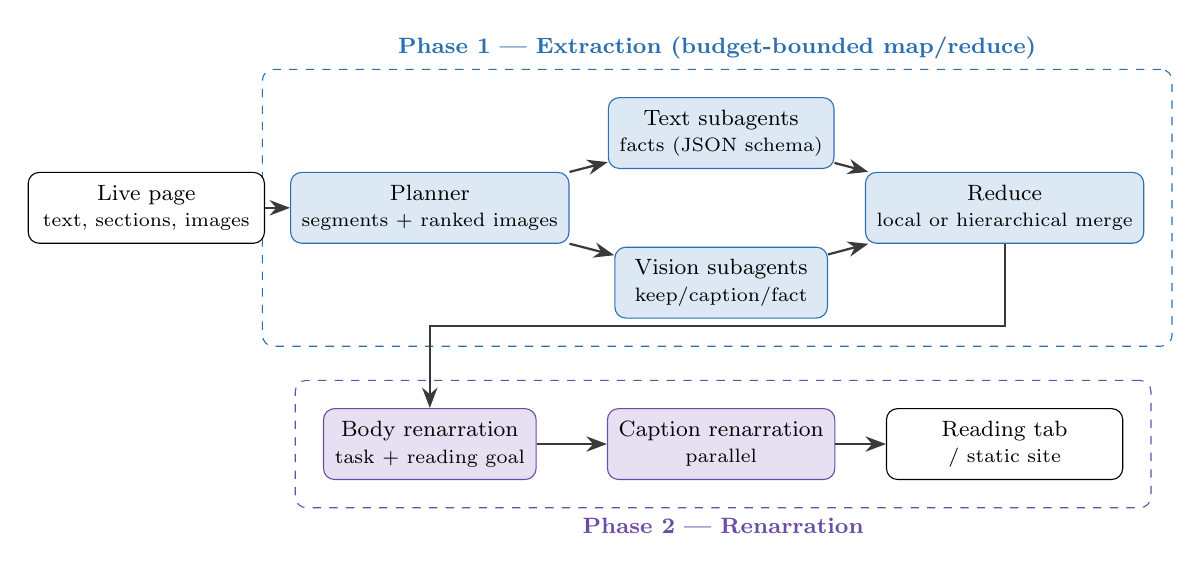
\begin{tikzpicture}[
  every node/.style={font=\footnotesize},
  stage/.style={draw, rounded corners, align=center, minimum height=0.9cm, minimum width=3.0cm, inner sep=4pt, fill=white},
  ex/.style={draw=cExtractB, fill=cExtract, rounded corners, align=center, minimum height=0.9cm, minimum width=2.7cm, inner sep=4pt},
  re/.style={draw=cRenarB, fill=cRenar, rounded corners, align=center, minimum height=0.9cm, minimum width=2.7cm, inner sep=4pt},
  ar/.style={-{Stealth[length=2.6mm]}, thick, draw=cEdge}
]
% Input
\node[stage] (page) at (0,0) {Live page\\\scriptsize text, sections, images};

% Extraction column
\node[ex] (plan) at (3.6,0) {Planner\\\scriptsize segments + ranked images};
\node[ex] (text) at (7.3,0.95) {Text subagents\\\scriptsize facts (JSON schema)};
\node[ex] (vis) at (7.3,-0.95) {Vision subagents\\\scriptsize keep/caption/fact};
\node[ex] (red) at (10.9,0) {Reduce\\\scriptsize local or hierarchical merge};

% Renarration row
\node[re] (body) at (3.6,-3.0) {Body renarration\\\scriptsize task + reading goal};
\node[re] (cap) at (7.3,-3.0) {Caption renarration\\\scriptsize parallel};
\node[stage] (out) at (10.9,-3.0) {Reading tab\\\scriptsize / static site};

\draw[ar] (page) -- (plan);
\draw[ar] (plan) -- (text);
\draw[ar] (plan) -- (vis);
\draw[ar] (text) -- (red);
\draw[ar] (vis) -- (red);
\draw[ar] (red) -- ++(0,-1.5) -| (body);
\draw[ar] (body) -- (cap);
\draw[ar] (cap) -- (out);

% Phase labels
\begin{scope}[on background layer]
\node[draw=cExtractB, dashed, rounded corners, fit=(plan)(text)(vis)(red), inner sep=10pt, label={[cExtractB]above:\textbf{Phase 1 --- Extraction (budget-bounded map/reduce)}}] {};
\node[draw=cRenarB, dashed, rounded corners, fit=(body)(cap)(out), inner sep=10pt, label={[cRenarB]below:\textbf{Phase 2 --- Renarration}}] {};
\end{scope}
\end{tikzpicture}
\caption{Two-phase pipeline. Extraction plans the page, runs text and vision
subagents in parallel under a single run budget, and reduces their output to
structured facts; renarration writes the body and image captions in parallel and
opens a reading tab or static site.}
\label{fig:pipeline}
\end{figure}

\section{User Interface Design}
Clear exposes several lightweight surfaces. The toolbar \emph{popup} offers
quick actions---open the overlay, view the last extraction, export a static site,
and open settings---and a \emph{side panel} mirrors the overlay entry point. The
\emph{selection card} appears as a glass card above selected text, labeled with
the word count and the active task ``lens,'' and offers Good/Off/Try-again
actions; it is an ARIA live region so assistive technology announces the result.
The \emph{document overlay} is rendered into a Shadow DOM to isolate it from host
styles and contains the reading-goal panel and the chatbot; its open state is
kept per tab. The \emph{options page} provides task create/edit/delete, a system
prompt-template editor with an effective-prompt preview, the anonymous study user
ID, and the research-logging toggle. Three \emph{viewer} pages render the
extracted page knowledge (with Re-extract, Copy JSON, Static site, and Renarrate
actions), the final renarrated reading page, and the research dashboard (Overview,
Conversations, Feedback, Preferences, Logs, and Export tabs).

\chapter{IMPLEMENTATION AND TESTING}
\label{ch:impl}

\section{Implementation}
The extension is written in vanilla JavaScript using ES modules and the Chrome
Manifest V3 APIs. Table~\ref{tab:stack} lists the technology stack.

\begin{table}[thbp]
\vskip\baselineskip
\caption[Technology stack]{Technology stack.}
\begin{center}
\begin{tabular}{@{}lll@{}}
\toprule
\textbf{Component} & \textbf{Technology} & \textbf{Purpose} \\
\midrule
Language & JavaScript (ES modules) & Application logic \\
Platform & Chrome Extension (Manifest V3) & Browser integration \\
LLM backend & OpenAI Responses API (\texttt{gpt-5.5}) & Text renarration and image understanding \\
Structured output & OpenAI strict JSON schema & Facts, image curation, goal extraction \\
Bundler & Vite 8 & Bundles the MV3 service worker \\
Config storage & \texttt{chrome.storage} sync / local & Settings and pipeline state \\
Research storage & IndexedDB (on-device) & Chat, feedback, logs, preferences \\
Tooling & ESLint, Prettier, knip, Vitest & Lint, format, dead-code, tests \\
CI & GitHub Actions (Node 20) & Build, lint, and test \\
\bottomrule
\end{tabular}
\label{tab:stack}
\end{center}
\end{table}

The OpenAI client centralizes request construction. It validates the API key,
sends \texttt{store: false}, selects the text or vision model automatically based
on whether image inputs are present, and strips request parameters a given model
rejects (retrying once if the API names an unsupported parameter). For
structured calls it requests strict JSON-schema output and, if a long page
overflows the token budget and truncates the JSON, retries once with double the
budget before surfacing a clear error. The renarration call uses a generous
output budget (16{,}000 tokens) with low reasoning effort, and runs the body
prose and the image-caption renarration in parallel. The API key is supplied at
build time through \texttt{VITE\_OPENAI\_API\_KEY}; as documented in
\texttt{SECURITY.md}, anything bundled into a client-side extension is
extractable, so the project mitigates this with key rotation, usage caps, and a
gitignored \texttt{.env}, and tracks a server-proxy/per-user-key approach as
future work.

\section{Testing}
Verification relies on a CI pipeline and a focused unit-test suite rather than a
large end-to-end harness. The GitHub Actions workflow runs on every push and pull
request and executes \texttt{npm install}, \texttt{npm run build},
\texttt{npm run lint}, and \texttt{npm test} on Node 20. Unit tests
(\texttt{popup-stub.test.js}, \texttt{sidepanel-stub.test.js}, and
\texttt{src/utils/id.test.js}) run under Vitest, \texttt{knip} checks for unused
files and exports, and \texttt{git diff --check} catches whitespace defects.
Runtime correctness is reinforced by the design itself---the budget ceilings,
run lock, transient-error and truncation retries, and the surfaced coverage
warnings---and by manual inspection through the extracted-content and dashboard
viewers.

\section{Deployment}
The extension runs entirely within Chrome, so there is no server component or
containerization. A developer copies \texttt{.env.example} to \texttt{.env} and
sets \texttt{VITE\_OPENAI\_API\_KEY}, runs \texttt{npm install} and
\texttt{npm run build} to produce \texttt{build/background-entry.js}, and loads
the repository root as an unpacked extension at \texttt{chrome://extensions} with
Developer Mode enabled. Updating the code only requires rebuilding the service
worker and reloading the unpacked extension.

\chapter{RESULTS}
As of this milestone, all core features are implemented and functional. Text
selections are renarrated in the on-page card; whole pages are extracted into
structured facts and renarrated into a clean reading tab; images are curated and
their captions renarrated by the vision step; pages can be exported as
self-contained static sites with images embedded as data URIs; the chatbot
produces a structured reading goal that steers subsequent renarration; the four
default tasks and the system prompt template are editable from the options page;
and research data is captured on-device with feedback and JSON/CSV export from the
dashboard. The continuous-integration pipeline (build, lint, test) passes on
Node~20, and the security posture---key handling, host-permission rationale, and
content-script isolation---is documented in \texttt{SECURITY.md}.

Concrete, repository-grounded parameters characterize the system's current
behavior: extraction is bounded by a 220{,}000\,ms / 350{,}000-token / 8.5\,MB
run budget; the renarration body call uses a 16{,}000-token output budget; and the
default request timeout is 120\,s. \textbf{A formal quality evaluation has not yet
been conducted.} The planned evaluation for the remainder of the project
comprises: a renarration-quality comparison across the four default tasks scored
on appropriateness, faithfulness, clarity, and tone; an extraction
budget/coverage analysis measuring how often pages hit each ceiling and how many
items are skipped; a static-site fidelity check on visually complex pages; and a
small user study that mines the on-device feedback and preference data to assess
real-world renarration quality.

\chapter{CONCLUSION}
This report presented Clear, a Manifest V3 Chrome extension for personalized web
page renarration built on the OpenAI Responses API. Its defining choices are a
clean separation between a budget-bounded, map/reduce \emph{extraction} phase and
a goal-driven \emph{renarration} phase; decoupled vision-based image curation; a
prompt and task system that lets users reshape output without code changes; a
reading-goal chatbot that personalizes results; and a fully on-device research
store that keeps telemetry private. The core system is implemented and functional,
and its reliability is enforced by explicit budgets, locks, and retries rather
than by assumption.

The remaining work for the final report is to conduct the formal quality and
coverage evaluation described in Chapter~8, run a small user study using the
already-collected feedback data, and address the documented API-key exposure by
moving credentials out of the shipped bundle. Citation examples:
\cite{kintsch}, \cite{openai}, \cite{mv3}, \cite{mapreduce}. Footnote
example\footnote{More details: {\url{https://www.cmpe.boun.edu.tr/}}}. Referring
to figures and tables: Figure~\ref{fig:pipeline}, Table~\ref{tab:stack}.

\begin{thebibliography}{99}
\bibitem{kintsch} W. Kintsch, \textit{Comprehension: A Paradigm for Cognition}. Cambridge University Press, 1998.
\bibitem{openai} OpenAI, ``OpenAI API --- Responses API and structured outputs,'' OpenAI Platform Documentation, 2025. [Online]. Available: \url{https://platform.openai.com/docs}.
\bibitem{mv3} Google, ``Chrome Extensions --- Manifest V3,'' Chrome for Developers, 2024. [Online]. Available: \url{https://developer.chrome.com/docs/extensions}.
\bibitem{wcag} W3C, ``Web Content Accessibility Guidelines (WCAG) 2.2,'' W3C Recommendation, 2023.
\bibitem{mapreduce} J. Dean and S. Ghemawat, ``MapReduce: Simplified data processing on large clusters,'' in \textit{Proc. OSDI}, pp. 137--150, 2004.
\bibitem{flesch} R. Flesch, ``A new readability yardstick,'' \textit{Journal of Applied Psychology}, vol. 32, no. 3, pp. 221--233, 1948.
\bibitem{parrots} E. M. Bender, T. Gebru, A. McMillan-Major, and S. Shmitchell, ``On the dangers of stochastic parrots: Can language models be too big?,'' in \textit{Proc. ACM FAccT}, pp. 610--623, 2021.
\bibitem{indexeddb} W3C, ``Indexed Database API 3.0,'' W3C Working Draft, 2024.
\bibitem{vite} Vite, ``Vite --- Next generation frontend tooling,'' 2024. [Online]. Available: \url{https://vitejs.dev}.
\end{thebibliography}

\appendix
\chapter{REPOSITORY MAP AND BUILD VERIFICATION}
The complete source is contained in the project repository. The principal
modules are: \texttt{src/background/} (service-worker entry and message router);
\texttt{src/handlers/} (\texttt{simple.js}, \texttt{chatbot.js});
\texttt{src/page-flow/} (\texttt{extract-page.js}, \texttt{renarrate-page.js},
\texttt{build-static-site.js}, \texttt{orchestrator.js});
\texttt{src/utils/} (\texttt{openai-client.js}, \texttt{llm-dispatch.js},
\texttt{renarration.js}, \texttt{prompt-loader.js}, \texttt{storage-helpers.js},
\texttt{research-store.js}); \texttt{src/prompts/} (\texttt{system.md},
\texttt{chatbot-system.md}, \texttt{goal-extraction.md}); the content scripts
(\texttt{content.js}, \texttt{clear-overlay.js}, \texttt{clear-shared.js}); the UI
pages (\texttt{popup.html}, \texttt{sidepanel.html}, \texttt{options.html} /
\texttt{options.js}); and the \texttt{viewers/} pages. The build and verification
commands documented in the repository README are:
\texttt{npm install}, \texttt{npm run build}, \texttt{npm run lint},
\texttt{npm test}, \texttt{npm run knip}, and \texttt{git diff --check}.

\end{document}
